\section{\vt\ Usage Study}

In this section, we present the empirical study on how 
academic people use \vt. 
We will first discuss how we collect academic papers to conduct the study, 
and then we will present our findings and implications. 

\subsection{Methodology}

We leverage published academic papers to understand 
how academic people use \vt,
since published papers usually contain detailed descriptions 
about how the authors use \vt\ in their projects, if \vt\ is involved. 

To collect academic papers, we search for keyword ``\vt'' in Google Scholar. 
In total, we find 101 conference papers published in the last ten years.
We then manually inspect descriptions related to \vt\ in these papers. 
In 87 papers, the authors either use \vt\ 
to build a data set for their evaluation~\cite{ford2009analyzing,android-1,email-vt-1,kharraz2016unveil} 
or leverage querying \vt\ as one building block of their
techniques~\cite{vt-component-1,vt-component-2,vt-component-3}. 
These 87 papers are targets of our \vt{} usage study. 
For the left 14 papers, their authors just discuss \vt\ as a part 
of technical background~\cite{not-use-1,bayer2009scalable,jiang2012dissecting}, and 
they do not use \vt\ in building their techniques or evaluation. 
Therefore, we ignore these papers in our study. 


\begin{figure}%
\centering
\subfigure[Conference]{%
\label{fig:conference}%
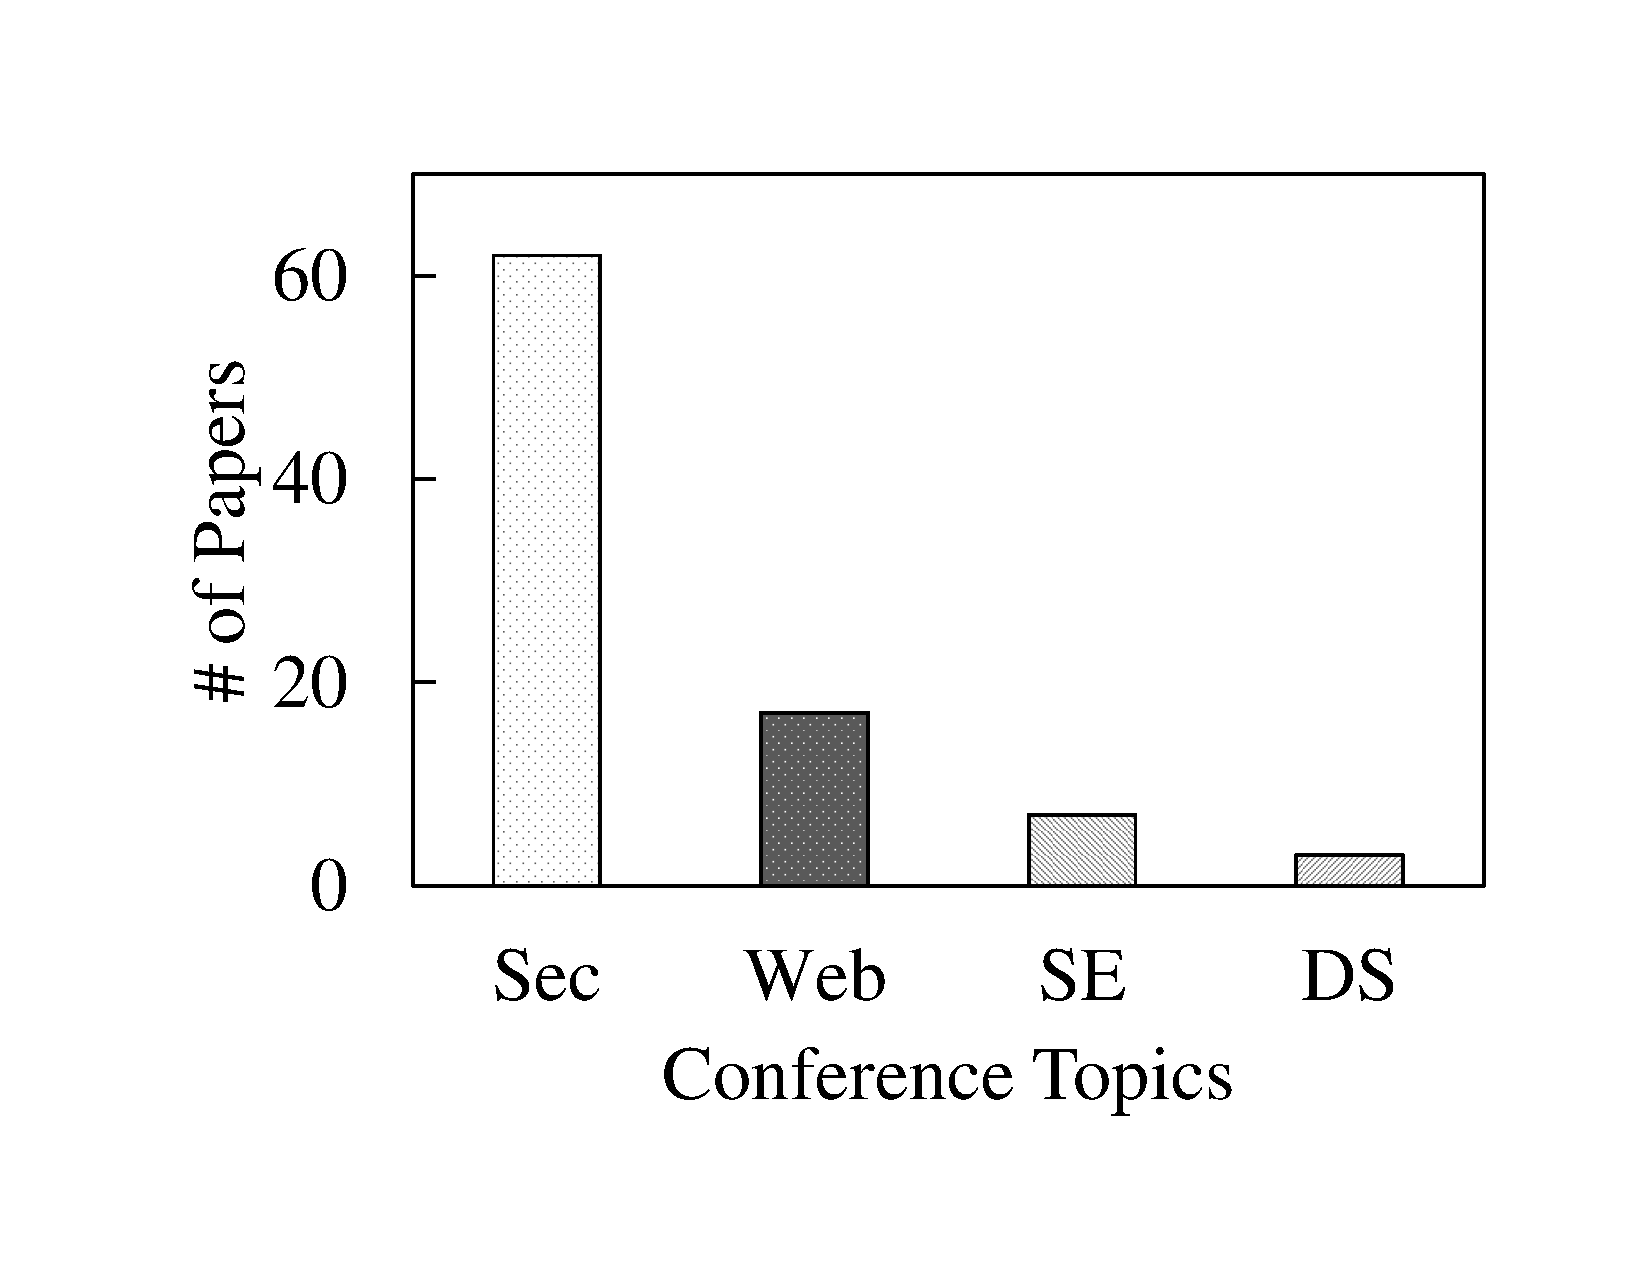
\includegraphics[width=1.45in]{figure/literature-confs}}%
\qquad
\subfigure[Publication Year]{%
\label{fig:year}%
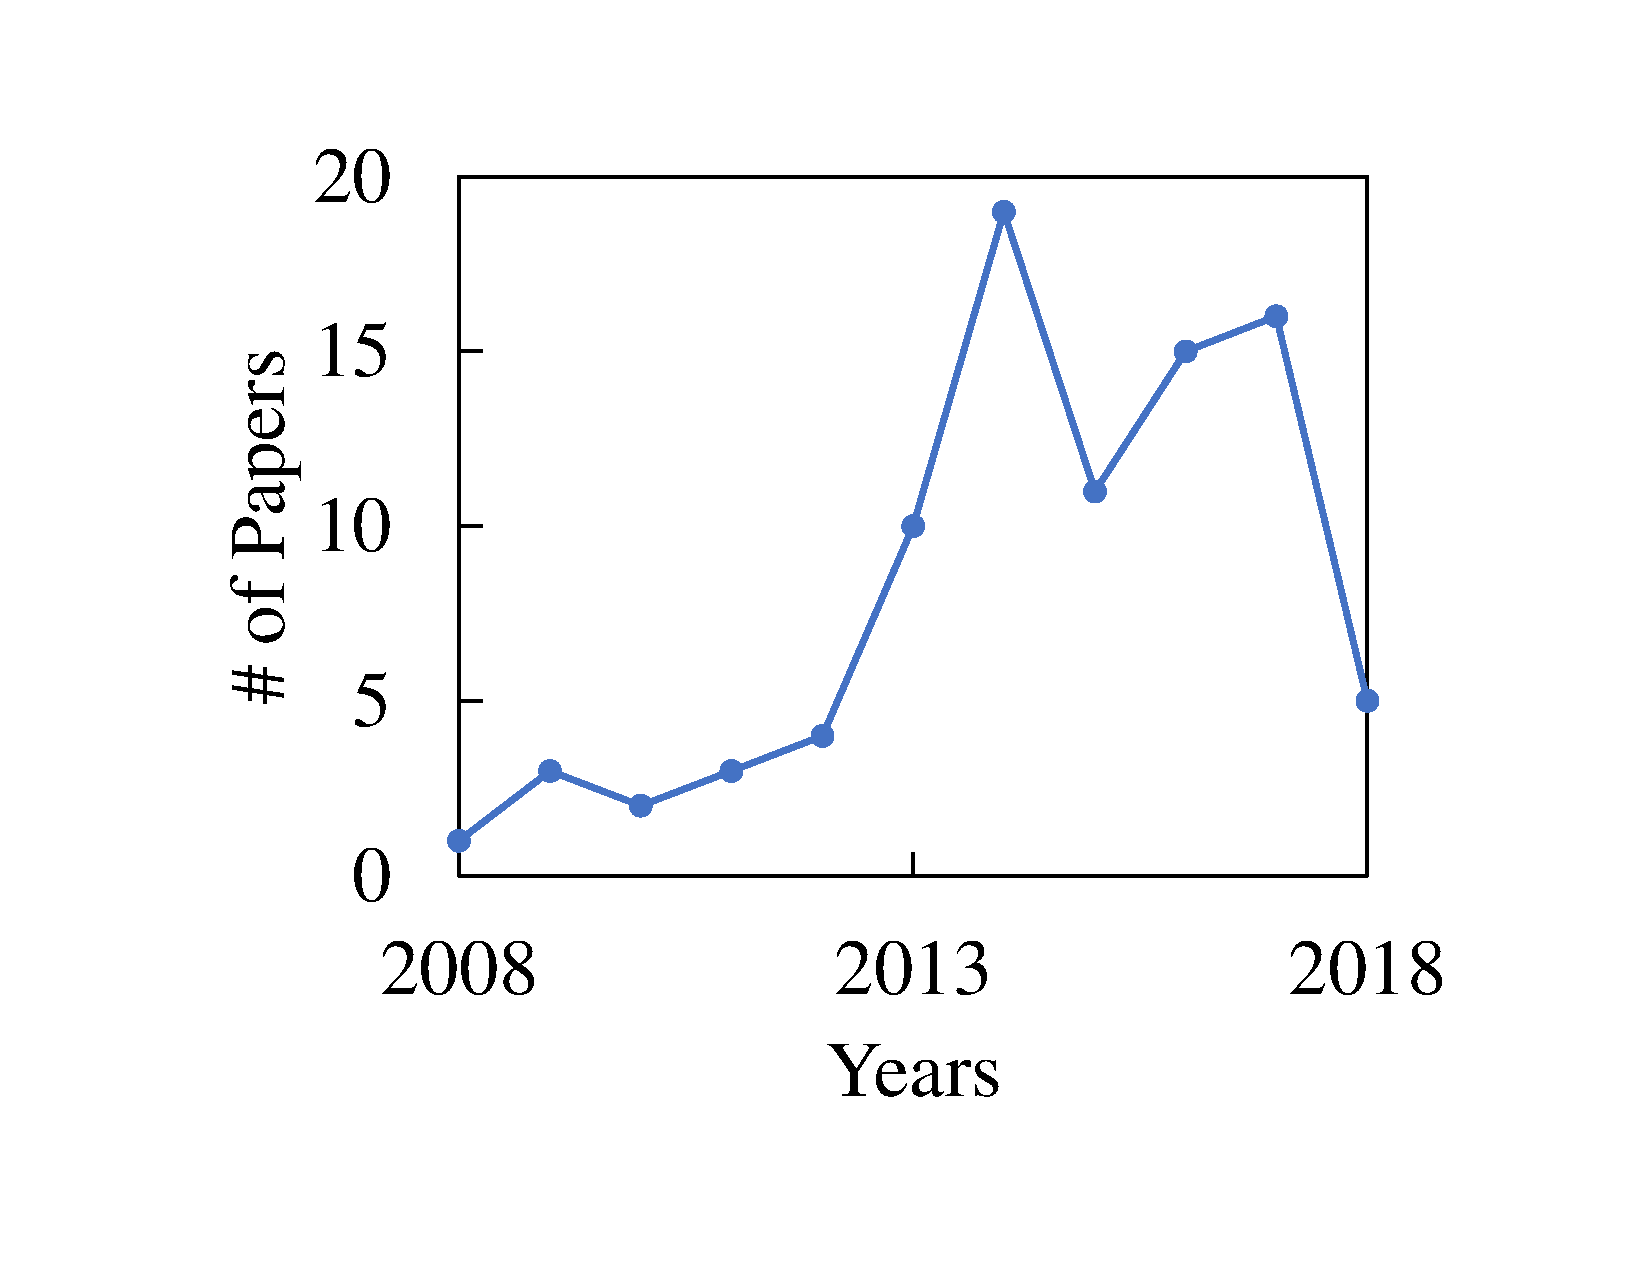
\includegraphics[width=1.45in]{figure/literature-years}}%
\mycaption{fig:char}
{Characteristics of our studied papers.}
{Sec: Security, DS: Data Science and SE: Software Engineering.}
\end{figure}




As shown in Figure~\ref{fig:conference}, 
our collected papers mainly come from famous academic conferences 
in four research areas, security, software engineering, data science, and web. 
For example, in total, we study 62 papers published in security conferences,
and 28 of them come from the top four security conferences, 
IEEE S\&P, CCS, Usenix Security, and NDSS.
As shown in Figure~\ref{fig:year}, 
we have at least one studied papers 
published in each year from 2008 to 2018. 
19 studied papers are published in 2014, 
and it is the year with largest number. 
Our studied papers cover different types of malware, 
such as Android APK~\cite{android-1,arp2014drebin,huangvt2016bigdata}, 
Portable Executable (PE) files~\cite{bayer2009scalable,pe-vt-1,pe-vt-2}, 
Flash~\cite{ford2009analyzing,wressnegger2017looking}, 
PDF~\cite{pdf-vt-1,carmony2016extract}, and so on. 
To sum up, we believe our studied paper is a representative data set 
to understand how academic people use \vt{}. 

\subsection{Findings and Implications}
We mainly want to answer two questions through our study.
First, \vt{} applies multiple antivirus engines to scan every submitted file, 
and returns all detection results to user.
Different engines may disagree with each other.
We want to understand how academic users aggregate results from different vendors,
and make the decision about whether a submitted file is benign for malicious. 
Second, \vt{} keeps updating antivirus engines. 
Intuitively, detection results could change when the same file is submitted twice.
We want to know whether or not academic users consider 
possible result changes on \vt{} over time.   
 

\noindent{\underline{How detection results are merged?}}
For 72 out of 89 (80.89\%) studied papers, 
their authors leverage a threshold to decide whether a submitted file is 
malicious or not. 
The threshold can either be a absolute number, 
or a ratio of the number of engines with malicious labels over all engines.
There are 26 studied papers, 
whose authors consider a submission is malicious, 
if any vendor label it as malware. 
For another {\color{red} XXX} papers, their authors 
use a absolute threshold number that is larger than one. 
Authors of {\color{red} XXX} papers use a ratio as their threshold. 
For the left 17 papers, their descriptions about how to merge results 
is not clear enough for us to study. 


\noindent{\underline{Whether possible changes are considered?}}





There several issues that researchers need to consider in using the results. 
First, researchers could collect detection results from multiple vendors. 
It is necessary to aggregate the results into one as the label of malware or benign for some works. 
We would like to know how researchers aggregate them. 
Second, the detection results could change over time and it is more reliable to collect the results from \vt\ during a period of time. 
We would also like to know the practice on collecting results from \vt\ over time. 
Thrid, vendors could have different impacts. 
It is also interesting to know whether and how researchers considered the different impacts of vendors.

%Last but not least, it is worth considering how we merge results from different vendors. 
First, we look at how researchers merge detection results. 
In most cases, researchers get results from more than 40 or 50 vendors and merge the results as one for their dataset. 
There are mainly two ways of merging: 1) considering a submission as malicious if any vendor can detect; 2) considering a ratio or a threshold for the number of vendors. 
For instance, Ford et al. \cite{ford2009analyzing} report it as malicious as long as there is a vendor reporting malicious
towards a file, while Carmony et al. use a threshold of 15 files. 
Among the 89 papers, 26 papers (29.2\%) use the first way and 46 papers  (51.7\%) use the second way. 
The rest 17 papers (19.1\%) do not mention how they merge results from different vendors.

Second, there are only 4 papers (4.5\%) consider that the detection results could change over time, and collect the results from \vt\ during a period of time. 
The length of time could vary from several days \cite{kharraz2016unveil, rajab2013camp} to months \cite{neeles, wressnegger2017looking}. 

Third, among the 89 papers, only 8 papers (9.0\%) consider that different vendors shall have different impact. 
Most of them pick out three to more than ten vendors to discuss their impact, because of their influence in industry or good performance on detection rate. 
For instance, Arp et al. \cite{arp2014drebin} inspected the output of ten vendors and list their detection rate anonymously. 
In addition, all of the papers treat the vendors equally. %Thomas et al. \cite{thomas2015ad} listed detection rate of 3 vendors. 
\subsection{Findings}
a. Do not wait until results become stable

b. Treat vendors equally

\subsection{Discussion}
What if the current usage is not correct? 
